
\clearpage

\section {Comparison between $\nu$ and $\bar{\nu}$ only contours with the Run 1-7c dataset}
\label{sec:results_run17c_nu_nubar}

In fig.~\ref{fig:contours_nu_nubar_only_run17c} the contours of $\sin^2 \theta_{13}$ Vs $\delta_{CP}$
obtained by analyzing either the $\nu$ or $\bar{\nu}$ event samples in the Run 1-7c data set are compared.
Both the $\nu$-only and $\bar{\nu}$-only contours are in good agreement with the reactor measurement
in the region of the parameters approximately close to $\delta_{CP} = -\pi/2$ and normal hierarchy.
It is also clear that the $\bar{\nu}$-only contour is not statistically powerful enough to observe 
non-zero $\theta_{13}$ with good significance. 
Without analyzing the $\nu$ and $\bar{\nu}$ data simultaneously 
the region at $\delta_{CP} = \pi/2$ is not excluded at 90\% CL with constant $\Delta \chi^2$ method.

\begin{figure}
\center
%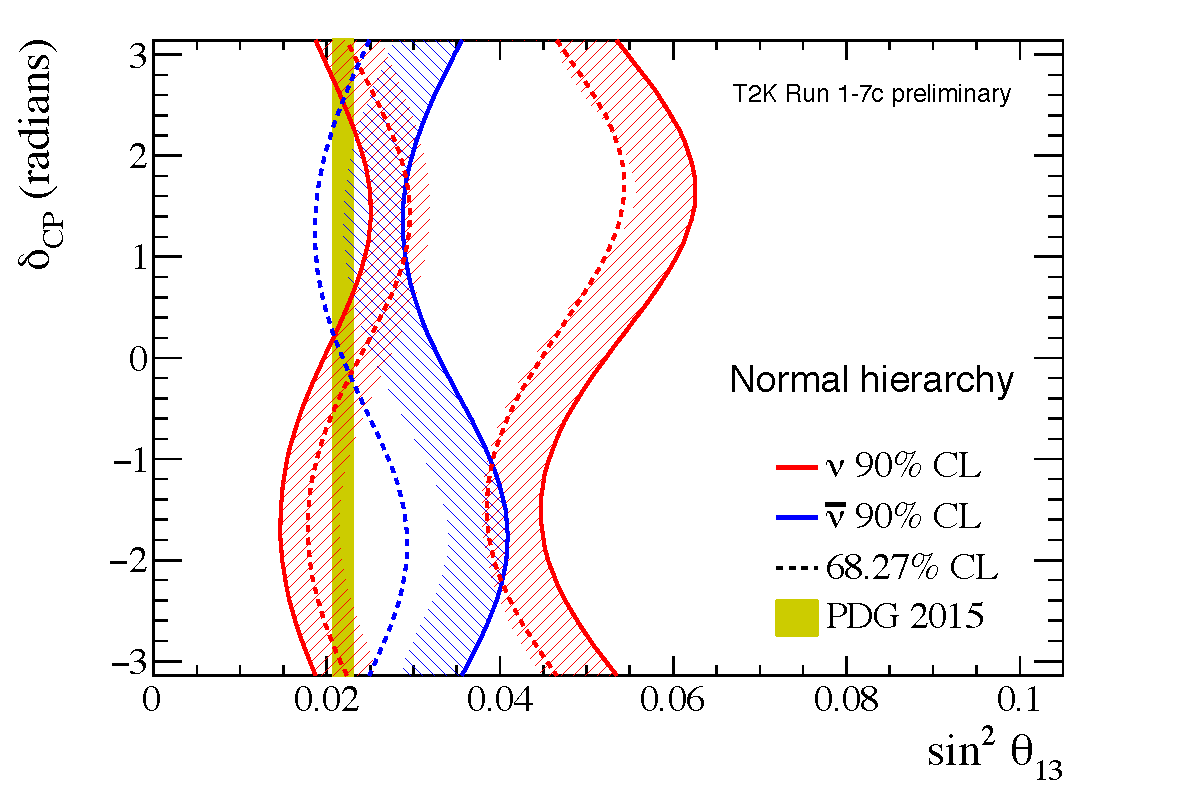
\includegraphics[width=0.9\textwidth]{./joint_plots/data_contours/Run17c/nu_vs_nuebar/NH_90_exclusion_w68.pdf}
%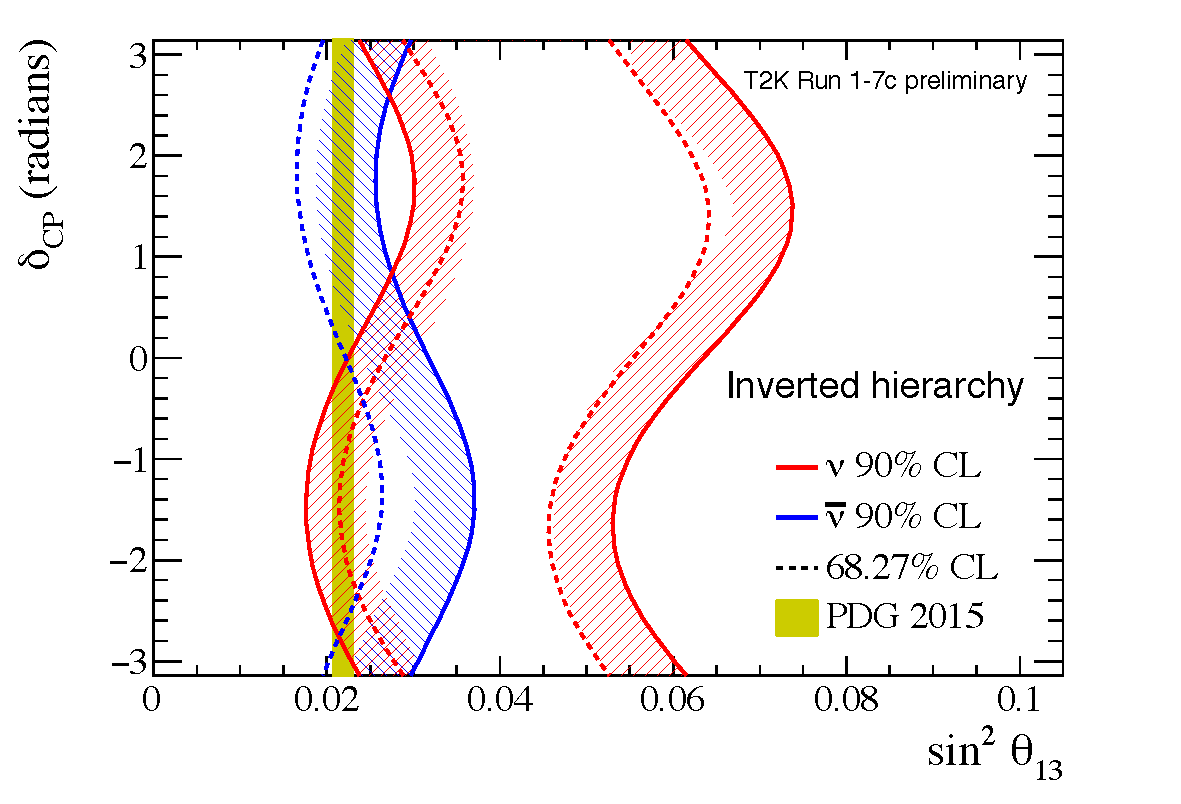
\includegraphics[width=0.9\textwidth]{./joint_plots/data_contours/Run17c/nu_vs_nuebar/IH_90_exclusion_w68.pdf}
\begin{subfigure}[b]{0.49\textwidth}
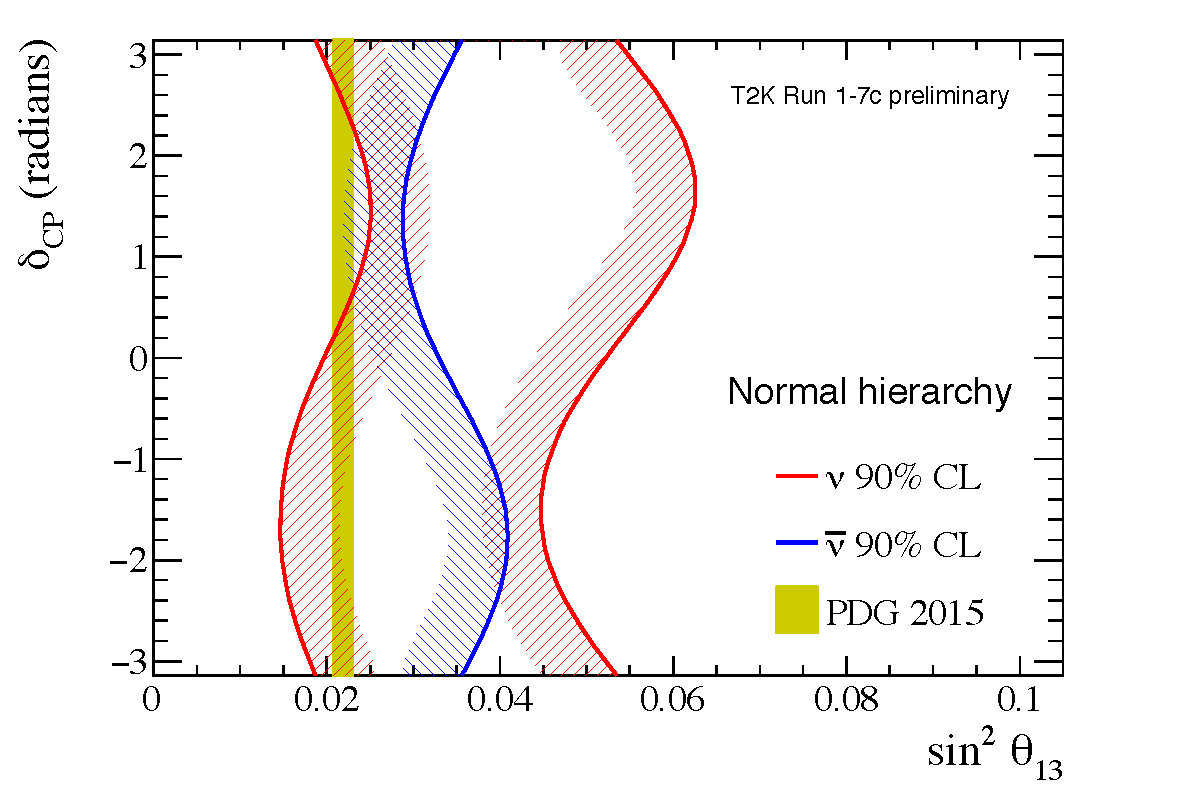
\includegraphics[width=0.9\textwidth]{./joint_plots/data_contours/Run17c/nu_vs_nuebar/NH_90_exclusion.pdf} 
\caption{Only 90\% CL - Normal Hierarchy}
\end{subfigure}
\begin{subfigure}[b]{0.49\textwidth}
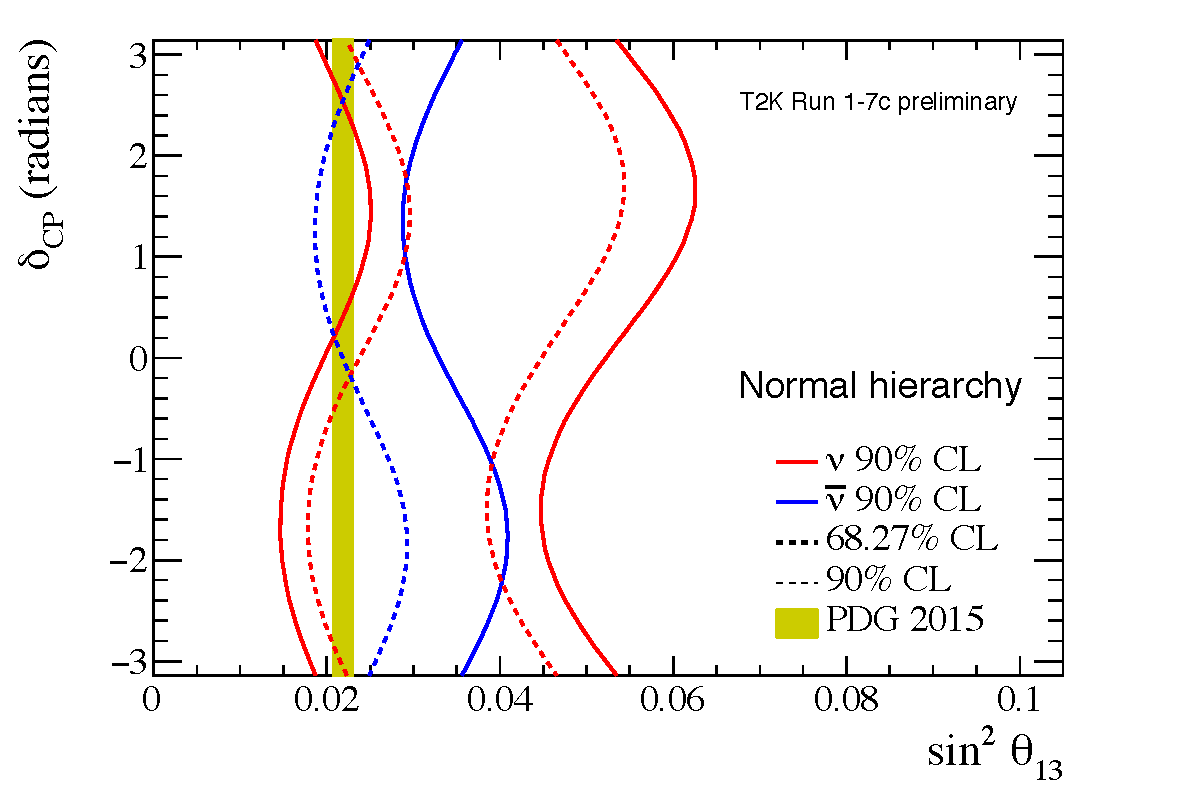
\includegraphics[width=0.9\textwidth]{./joint_plots/data_contours/Run17c/nu_vs_nuebar/NH.pdf} \\
\caption{68\% CL and 90\% CL - Normal Hierarchy}
\end{subfigure}
\begin{subfigure}[b]{0.49\textwidth}
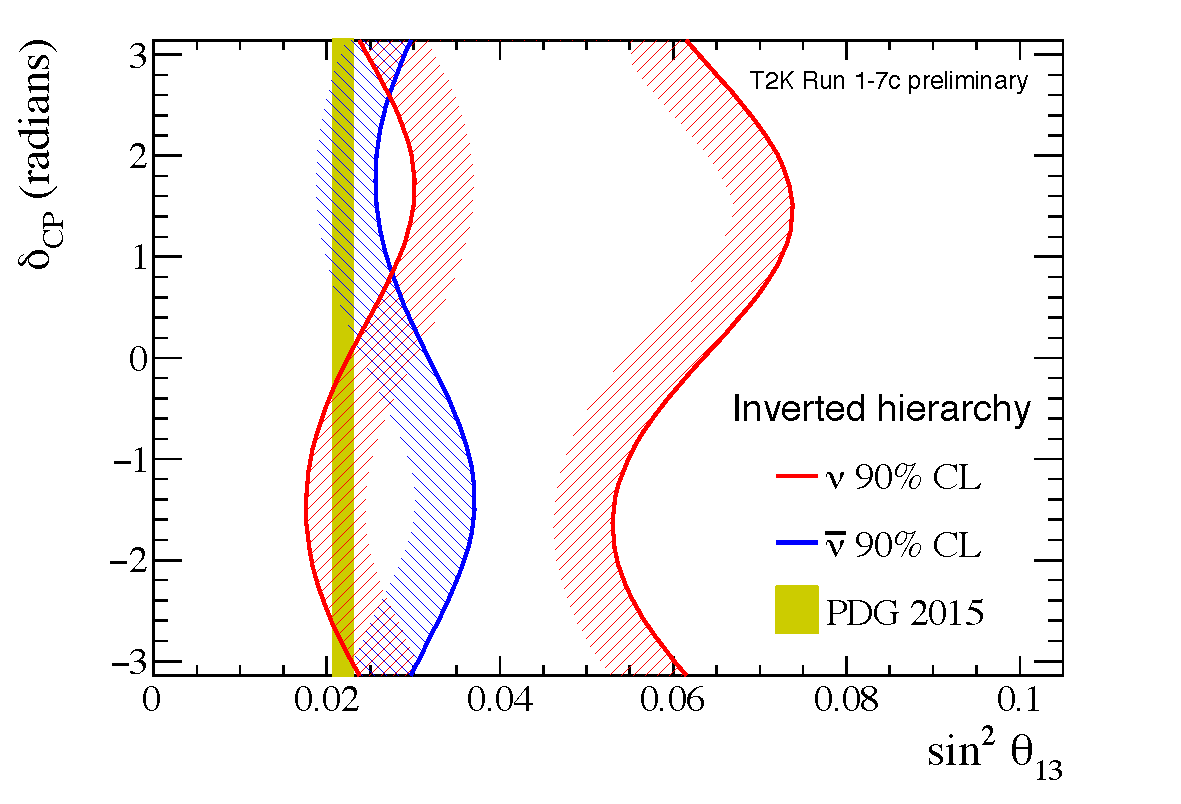
\includegraphics[width=0.9\textwidth]{./joint_plots/data_contours/Run17c/nu_vs_nuebar/IH_90_exclusion.pdf}
\caption{Only 90\% CL - Inverted Hierarchy}
\end{subfigure}
\begin{subfigure}[b]{0.49\textwidth}
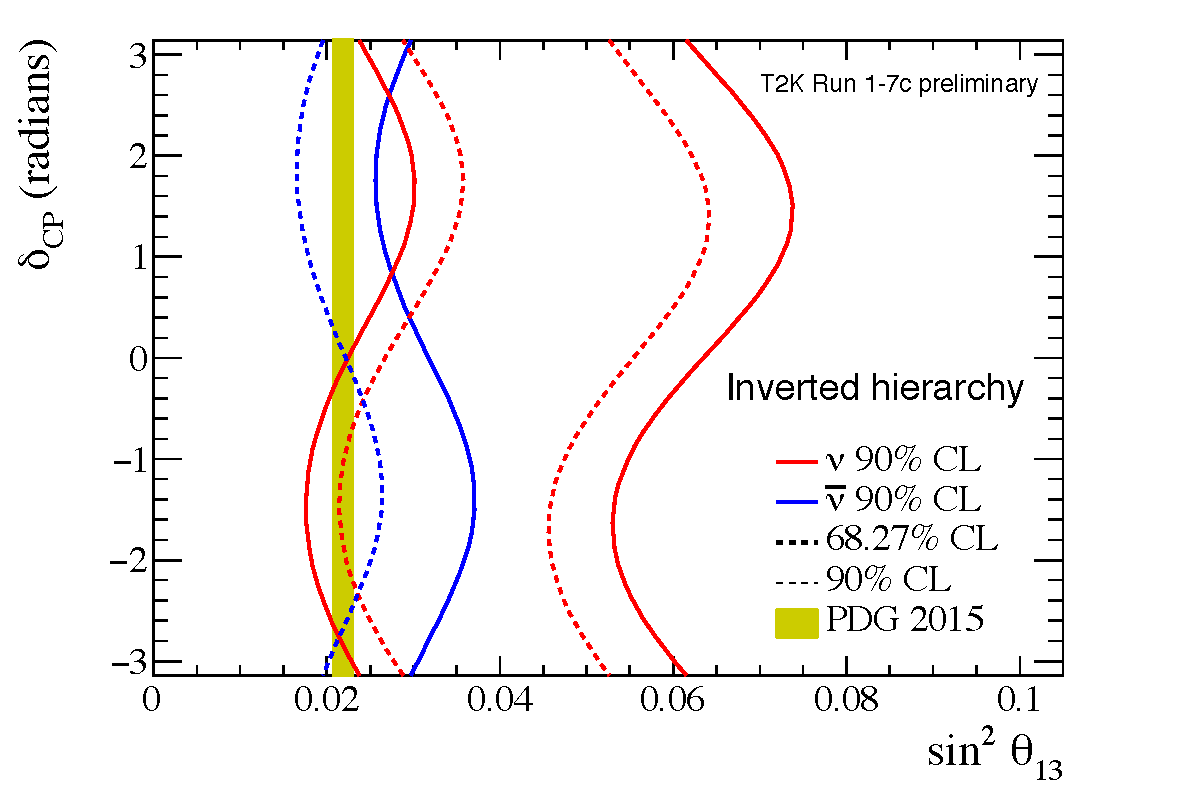
\includegraphics[width=0.9\textwidth]{./joint_plots/data_contours/Run17c/nu_vs_nuebar/IH.pdf}
\caption{68\% CL and 90\% CL - Inverted Hierarchy}
\end{subfigure}
\caption {
The contours of $\sin^2 \theta_{13}$ Vs $\delta_{CP}$ T2K only,
obtained by analyzing only either the $\nu$ only or the $\bar{\nu}$ only Run 1-7c data set are compared
for both hierarchies. 
The yellow band corresponds to the reactor value of the PDG 2015.
Depending on the figure, either 68\% and/or 90\% CL contours are shown.
In the left plots only 90\% CL contours are shown. The hatches show the allowed region.
In the right plots both the 68\% and 90\% CL contours are shown.
For $\bar{\nu}$-only the region on the left side of the blue lines is allowed, 
while for $\nu$-only the region between the red lines is allowed.    
}
\label{fig:contours_nu_nubar_only_run17c}
\end{figure}

